%                      Code_Saturne version 1.3
%                      ------------------------
%
%     This file is part of the Code_Saturne Kernel, element of the
%     Code_Saturne CFD tool.
%
%     Copyright (C) 1998-2007 EDF S.A., France
%
%     contact: saturne-support@edf.fr
%
%     The Code_Saturne Kernel is free software; you can redistribute it
%     and/or modify it under the terms of the GNU General Public License
%     as published by the Free Software Foundation; either version 2 of
%     the License, or (at your option) any later version.
%
%     The Code_Saturne Kernel is distributed in the hope that it will be
%     useful, but WITHOUT ANY WARRANTY; without even the implied warranty
%     of MERCHANTABILITY or FITNESS FOR A PARTICULAR PURPOSE.  See the
%     GNU General Public License for more details.
%
%     You should have received a copy of the GNU General Public License
%     along with the Code_Saturne Kernel; if not, write to the
%     Free Software Foundation, Inc.,
%     51 Franklin St, Fifth Floor,
%     Boston, MA  02110-1301  USA
%
%-----------------------------------------------------------------------
%
%%%%%%%%%%%%%%%%%%%%%%%%%%%%%%%%%%
%%%%%%%%%%%%%%%%%%%%%%%%%%%%%%%%%%
\section{Discr\'etisation}
%%%%%%%%%%%%%%%%%%%%%%%%%%%%%%%%%%
%%%%%%%%%%%%%%%%%%%%%%%%%%%%%%%%%%

On pose :

\begin{equation}\notag
\displaystyle\alpha_{ij}=\frac{\overline{FJ'}}{\overline{I'J'}} \text{\ d\'efini aux faces internes uniquement et}
\end{equation}
\begin{equation}\notag
\vect{u}_{K'} = \vect{u}_{K}+(\ggrad{\vect{u}})_K\text{.}\, \vect{KK'}\, \text{\ \`a l'ordre
1 en espace, pour ${K = I \,\text{ou}\, J}$}
\end{equation}

\begin{figure}[h]
\hspace*{1cm}\parbox{8cm}{%
\centerline{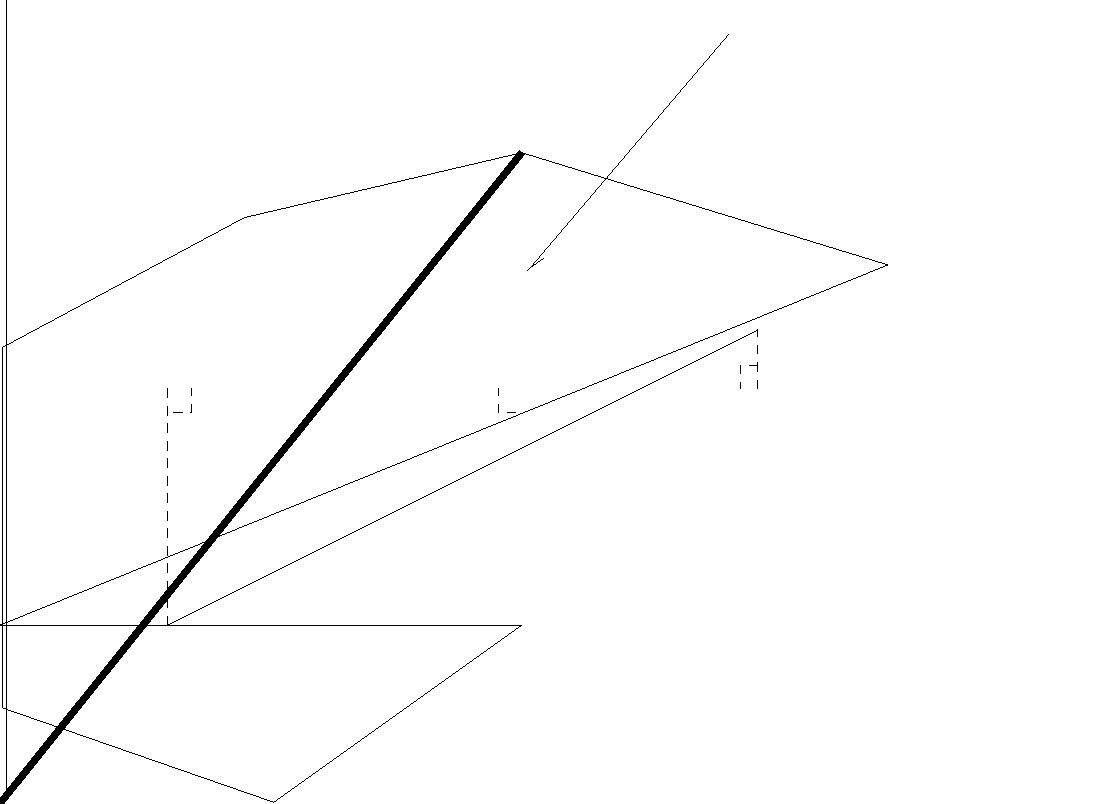
\includegraphics[height=4cm]{../Base/Navsto/Images/facette.pdf}}}
\parbox{8cm}{%
\centerline{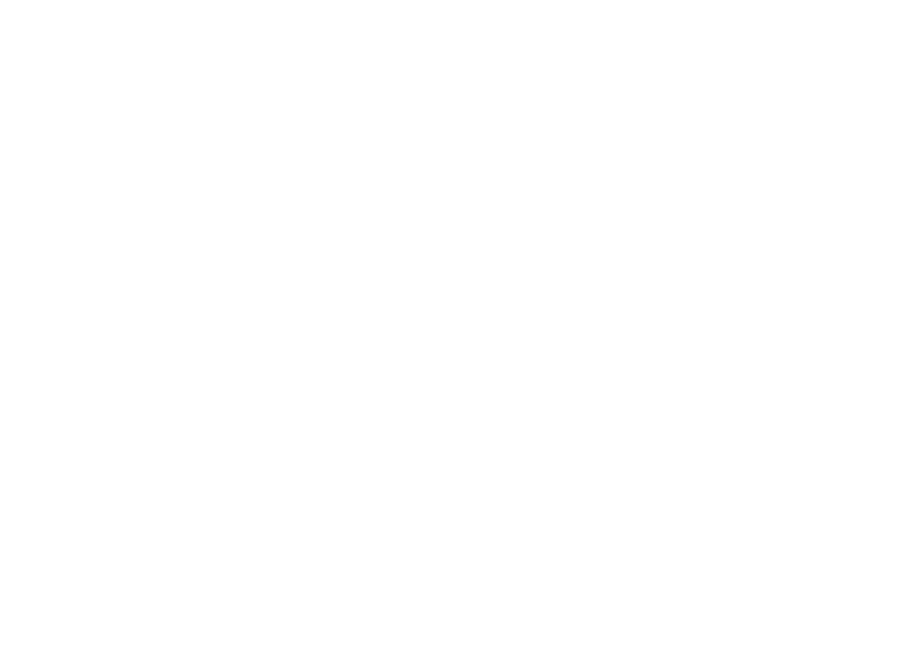
\includegraphics[height=4cm]{../Base/Navsto/Images/facebord.pdf}}}
\caption{\label{Base_Navsto_fig_geom}D\'efinition des diff\'erentes entit\'es
g\'eom\'etriques pour les faces internes (gauche) et de bord (droite).}
\end{figure}

\subsection{\bf M\'ethode \`a pas fractionnaires}
\subsubsection{\bf Introduction}
Une des m\'ethodes permettant de r\'esoudre num\'eriquement les \'equations de
Navier-Stokes est de d\'ecomposer les op\'erateurs s'y rattachant en
op\'erateurs moins complexes (qui peuvent \^etre trait\'es \`a l'aide d'algorithmes
efficaces), moyennant des sous-pas interm\'ediaires dans un m\^eme pas de
temps. Ici, deux sous-pas sont r\'ealis\'es : le premier reprend les
parties convective, diffusive et termes sources de l'\'equation de quantit\'e de mouvement et
constitue l'\'etape dite de pr\'ediction de la vitesse, le
second traite l'\'equation de continuit\'e et est
d\'esign\'e comme l'\'etape de correction de pression ou de projection de la vitesse.

\subsubsection{\bf \'Etape de pr\'ediction des vitesses}
La discr\'etisation en temps se fait en appliquant \`a la variable r\'esolue un $\theta$-sch\'ema au temps $n+\theta$ s'inspirant de la d\'emarche utilis\'ee pour l'\'equation de transport d'un scalaire\footnote{cf. \fort{covofi}}.\\ La vitesse au temps $n+1$ n'\'etant disponible qu'apr\`es l'\'etape de projection, c'est ici une vitesse pr\'edite au temps $n+1$ que l'on utilise pour interpoler :
\begin{equation}
\label{Base_Navsto_thetaschema}
\vect{\widetilde{u}}^{n+\theta} = \theta\, {\vect{\widetilde{u}}}^{n+1}+(1-\theta)\, \vect{u}^{n}
\end{equation}
Avec\footnote{Dans le cas o� $\theta = 1/2$, le pas de temps $\Delta t$ est suppos� uniforme en temps et en espace.} :
\begin{equation}
\left\{
\begin{array}{ll}
\theta = 1   & \text{Pour un sch\'ema de type Euler implicite d'ordre 1.}\\
\theta = 1/2 & \text{Pour un sch\'ema de type Cranck-Nicolson d'ordre 2.}\\
\end{array}
\right.
\end{equation}

Le champ de vitesse ${\vect{\widetilde{u}}^{n+1}}$ pr\'edit est alors obtenu par
:\\
$\bullet\ $ Lin\'earisation partielle de l'op\'erateur de convection engendrant
un d\'ecouplage des composantes de la vitesse.\\
$\bullet\ $ Explicitation de la pression.\\
$\bullet\ $ Explicitation ou extrapolation des grandeurs physiques ({\it i.e}
$\rho,\,\mu,\,Cp\,...$) et du flux de masse.\\
$\bullet\ $ Explicitation ou extrapolation des termes sources explicites au
temps $n+\theta_{S}$ tels que les contributions du gradient transpos\'e, de la
viscosit� secondaire, de la partie extradiagonale des pertes de charges, de la
masse inject�e $\Gamma\,\underline{u_i}$, ...\\
$\bullet$ Les termes sources implicites lin�aires par rapport � la vitesse
(termes sources utilisateurs implicite, partie diagonale des pertes de charge
$\tens{K_d}\,\underline{u}$, sources de masse $\Gamma\,\underline{u}$, etc...)
sont suppos�s pris au temps $n+\theta$ et sont rattach\'es au tenseur
$\tens{K}$\footnote{En r�alit�, les composantes de la vitesse �tant d�coupl�es,
seuls les termes lin�aires par rapport � la composante r�solue sont factoris�s de la
sorte. Les autres termes �tant trait�s comme des termes explicites. On pourra se
rapporter � \fort{preduv} pour plus de d�tail.}.\\

Par souci de clart�, on suppose qu'en l'absence d'indication, les propri�tes
physiques $\Phi\,=\,\rho,\,\mu\,...$ et le flux de masse $(\rho\vect{u})$ pris
respectivement aux instants $n+\theta_\Phi$ et $n+\theta_F$, o� $\theta_\Phi$ et
$\theta_F$ d�pendent des sch�mas en temps sp�cifiquement utilis�s pour ces
grandeurs\footnote{cf. \fort{introd}}.
\\
On r\'esout donc le syst\`eme suivant, apr�s r��criture des termes instationnaires � l'aide de la conservation de la masse :
\begin{equation}
\begin{array}{l}
\displaystyle
\rho\,\left(\displaystyle\frac{\vect{\widetilde{u}}^{n+1}-\vect {u}^{n}}{\Delta t}\right) +
\dive \,\left(\vect{\widetilde{u}}^{n+\theta} \otimes (\rho\vect{u})\right) =
\dive(\tens{\sigma}^{n+\theta})+\vect{TS}^{n+\theta_{S}}-\tens{K}^{n}\,\vect{u}^{n+\theta} +\vect{\widetilde{u}}^{n+\theta}\,\dive{(\rho\vect{u})}\\
\label{Base_Navsto_eq_prediction_continue}
\end{array}
\end{equation}
avec ~:
\begin{equation}
\begin{array}{l}
\displaystyle
\tens{\sigma}^{n+\theta}=\mu\,\,\ggrad\vect{\widetilde{u}}^{n+\theta}\underbrace{-P^{n-1+\theta}\tens{Id}+(\,\mu\,\,^{t}\ggrad\vect{u})^{n+\theta_{S}}- \frac{2}{3}\,(\,\mu\, \dive\,\vect{u})^{n+\theta_{S}}\tens{Id}}_{\text{termes sources explicites}}\\
\end{array}
\end{equation}

\subsubsection{\bf \'Etape de correction de la pression (ou projection des vitesses)}
Le champ de vitesse pr\'edit est {\it a priori} \`a divergence non nulle. La seconde
\'etape corrige la pression en imposant la nullit\'e de la contrainte
stationnaire pour la vitesse prise \`a l'instant ${t^{n+1}}$.
On r\'esout donc :
\begin{equation}\label{Base_Navsto_eq_correction_continue}
\left\{\begin{array}{l}
\displaystyle\frac{(\rho\vect{u})^{n+1}-(\rho\vect{\widetilde{u}})^{n+1}}{\Delta t} =
-\grad{\delta P^{n+\theta}} \\
\displaystyle
\dive(\rho\vect{u})^{n+1} = \Gamma\\
\end{array}\right.
\end{equation}

o\`u l'incr\'ement de pression $\delta P^{n+\theta}$ vaut~:
\begin{equation}
\delta P^{n+\theta}=P^{n+\theta}-P^{n-1+\theta}
\end{equation}
\minititre{Remarque}
Les quantit\'es $\rho$ et $\mu$ sont constantes lors de ces
deux \'etapes. Leur variation \'eventuelle est effectu\'ee au d�but du pas de temps suivant, apr�s r�actualisation des scalaires (temp�rature, fraction massique,...).

\subsection{\bf Discr\'etisation spatiale}
On int\`egre  classiquement sur les volumes de contr\^ole ${\Omega_i}$ (ou cellules) les
\'equations discr\'etis\'ees en temps.
\subsubsection{\bf \'Etape de pr\'ediction des vitesses}
\paragraph{\bf Second membre\\ }
Si l'on ne tient pas compte des termes de convection et de diffusion issus du $\theta$-sch�ma, les termes sources volumiques explicites de l'\'equation (\ref{Base_Navsto_eq_prediction_continue}) s'�crivent pour le syst\`eme portant sur la quantit� $(\vect{\widetilde{u}}^{n+1}-\vect {u}^{n})$ :\\
\begin{equation}\notag
\begin{array}{c}
\displaystyle
 -\grad P^{n-1+\theta} + \dive \left[ (\,\mu\,\,^{t}\ggrad\vect{u})^{n+\theta_{S}}- \frac{2}{3}\,(\,\mu\, \dive\,\vect{u})^{n+\theta_{S}}\tens{Id} \,\right]+\vect{TS}^{n+\theta_{S}}- \,\tens{K}^{n} \vect{u}^{n}+\vect{u}^{n}\,\dive{(\rho\vect{u})}\\
\end{array}
\end{equation}
Pour int\'egrer ces termes sur une cellule ${\Omega_i}$,  on multiplie leur valeur locale au centre par le volume de la cellule.

\paragraph{\bf Convection  \\}

Apr\`es d\'ecomposition de $\vect{\widetilde{u}}$ \`a l'aide de la relation (\ref{Base_Navsto_thetaschema}), l'int\'egration spatiale des parties convectives   $\theta\,{\dive\left(\vect{\widetilde{u}}^{n+1}\otimes (\rho \vect{u})\right)}$ et $(1-\theta)\,{\dive\left(
\vect{u}^{n}\otimes (\rho \vect{u})\right)}$ conduit � une somme de flux num\'eriques ${\vect{F}\,_{\,ij}}$ calcul\'es aux faces des cellules purement internes et de flux num\'eriques ${\vect{F}_{\,b_{ik}}}$ calcul\'es aux faces de bord du domaine $\Omega$.
Soient $Vois(i)$ l'ensemble des centres des cellules voisines de ${\Omega_i}$ et
$\gamma_b(i)$ l'ensemble des centres des faces de bord de ${\Omega_i}$, on a :

\begin{equation}\notag
\int_{\Omega_i}{\dive\left(\vect{u}\otimes (\rho \vect{u})\right)\, d\Omega} =
\sum_{j\in Vois(i)}{\vect{F}_{\,ij}((\rho \vect{u}), \vect{u})} \\
+\sum_{k\in {\gamma_b(i)}} {\vect{F}_{\,{b}_{ik}}((\rho \vect{u}),\vect{u})}
\end{equation}

en posant :
\begin{equation}
\vect{F}_{\,ij}((\rho \vect{u}), \vect{u}) = \left[{(\rho \vect{u})_{\,ij}} \text{.}\, \vect{S}_{\,ij}\right]
\ \vect{u}_{\,f,ij}
\end{equation}

\begin{equation}
{\vect{F}_{\,{b}_{ik}}}((\rho \vect{u}),\vect{u}) =  \left[{(\rho \vect{u})_{\,{b}_{ik}}} \text{.}\, \vect{S}_{\,{b}_{ik}}\right]\,{\vect{u}_f}_{\,{b}_{ik}}
\end{equation}
La valeur de ${\vect{F}_{\,ij}}$  d\'epend du type de sch\'ema num\'erique
choisi. Il en existe trois dans \CS \  :
\begin{tabular}{ll}
\multicolumn{2}{l}{$\bullet\ $un sch\'ema d\'ecentr\'e amont d'ordre 1 (upwind)~:}\\
&$\vect{F}_{\,ij}((\rho \vect{u}), \vect{u})=
\vect{F}^{\it{ amont}}_{\,ij}((\rho \vect{u}),\vect{u})$\\
o\`u :&$\vect{u}_{\,f,ij}=\vect{u}_{\,I}$ si $(\rho
\vect{u})_{\,ij}.\vect{S}_{\,ij}\,\geqslant 0$\\
&$\vect{u}_{\,f,ij}=\vect{u}_{\,J}$ si $(\rho
\vect{u})_{\,ij}.\vect{S}_{\,ij}\,< 0$ ,\\
\multicolumn{2}{l}{$\bullet\ $un sch\'ema centr\'e d'ordre 2:}\\
&$\vect{F}_{\,ij}((\rho \vect{u}), \vect{u})=
\vect{F}^{\text{\it{centr\'e}}}_{\,ij}((\rho\vect{u}),\vect{u})$\\
avec :&$\vect{u}_{\,f,ij}=
\alpha_{ij} \vect{u}_{\,I'}+(1-\alpha_{ij}) \vect{u}_{\,J'}$ et $\vect{u}_{K'} = \vect{u}_{K}+(\ggrad{\vect{u}})_K\text{.}\, \vect{KK'}$ pour ${K = I \,\text{ou}\, J}$\\
\multicolumn{2}{l}{$\bullet\ $un sch\'ema d\'ecentr\'e amont d'ordre 2 SOLU (Second Order Linear Upwind)~:}\\
&$\vect{F}_{\,ij}((\rho \vect{u}), \vect{u})=
\vect{F}^{\text{\it { SOLU}}}_{\,ij}((\rho \vect{u}),\vect{u})$ \\
\multicolumn{2}{l}{\begin {tabular}{lll}
avec :&$\vect{u}_{\,f,ij}=$&$
\vect{u}_{\,I} +\vect{IF}.\,(\ggrad\vect{u})_{\,I}$ \ si $(\rho
\vect{u})_{\,ij}.\vect{S}_{\,ij}\,\geqslant 0$\\
&&$\vect{u}_{\,J} + \vect{JF}.\,(\ggrad\vect{u})_J$  \ si $(\rho
\vect{u})_{\,ij}.\vect{S}_{\,ij}\,< 0$.
\end{tabular}}
\end{tabular}\\


La valeur de ${\vect{F}_{\,b_{ik}}}$ est calcul\'ee avec :\\
\begin{equation}
\begin{array}{ll}
{\vect{u}_f}_{\,{b}_{ik}} &=\vect{u}_{\,I}
\ \text{si $(\rho \vect{u})_{\,{b}_{ik}}\,.\,\vect{S}_{\,{b}_{ik}}\,\geqslant 0$}\\
&={\vect{u}_{\,{b}_{ik}}}
\  \text{si $(\rho \vect{u})_{\,{b}_{ik}}\,.\, \vect{S}_{\,{b}_{ik}}\,< 0$}
\end{array}
\end{equation}

avec ${\vect{u}_{\ {b}_{ik}}}$ valeur au bord donn\'ee directement par les
conditions aux limites.\\

\noindent\minititre{Remarque 2}
En centr\'e, on \'ecrit en r\'ealit\'e (\'egalit\'e
conservant l'ordre un en espace) :

\begin{equation}\notag
\vect{u}_{\,f,ij} = \alpha_{ij} \vect{u}_{\,I} +  (1-\alpha_{ij})
\vect{u}_{\,J} +
\frac{1}{2}\left[(\ggrad{\vect{u}})_I+(\ggrad{\vect{u}})_J\right] \text{.}\, \vect{OF}
\end{equation}

pour des raisons de stabilit\'e purement num\'erique.\\
\minititre{Remarque 3 }
Un test de pente (qui peut introduire des non lin\'earit\'es dans l'op\'erateur
de convection) permet de
basculer entre un sch\'ema d'ordre deux et le sch\'ema d\'ecentr\'e amont
d'ordre un.
De plus, en mode standard, on utilise en tout point une valeur de
$\vect{\widetilde{u}}_{\,f,ij}$ issue d'une moyenne barycentrique entre la valeur
d\'ecentr\'ee amont et la valeur d'ordre 2 (blending, sp�cifi� par l'utilisateur).
\paragraph{\bf Diffusion\\}
De m\^eme, les parties diffusives $\theta\,\,\dive(\mu\,\ggrad{\vect{\widetilde{u}}}^{n+1})$ et $(1-\theta)\,\,\dive(\mu \ggrad{\vect{u}}^{n})$ s'\'ecrivent :
\begin{equation}\notag
\int_{\Omega_i}{\dive(\mu\, \ggrad{\vect{u}}) d\Omega} =
\sum_{j\in Vois(i)}{\vect{D}_{\,ij}(\mu, \vect{u})}
+\sum_{k\in {\gamma_b(i)}} {\vect{D}_{\,{b}_{ik}}(\mu,\vect{u})}
\end{equation}
avec~:
\begin{equation}
\vect{D}_{\,ij}(\mu, \vect{u}) = \mu_{ij}
\frac{\vect{u}_{\,J'}-\vect{u}_{\,I'}}{\overline{I'J'}} S_{\,ij}
\end{equation}
et :
\begin{equation}
\vect{D}_{\,b_{ik}}(\mu, \vect{u}) = \mu_{\,b_{ik}}
\frac{\vect{u}_{\,b_{ik}}-\vect{u}_{\,I'}}{\overline{I'F}} S_{\,b_{ik}}
\end{equation}
en conservant les notations pr\'ec\'edentes et avec
${\vect{u}_{\,{b}_{ik}}}$ la valeur au bord donn\'ee directement par les conditions aux limites.\\
La viscosit\'e $\mu_{\,ij}$ \`a la face est calcul\'ee \`a l'aide des valeurs
aux centres selon une fonction $f$ donn\'ee :
\begin{equation}\notag
\mu_{\,ij} = f(\mu_I,\mu_J)
\end{equation}
qui est, soit une moyenne arithm\'etique~:
\begin{equation}
f(\mu_I,\mu_J)= \frac{1}{2}(\mu_I+\mu_J)
\end{equation}
soit une moyenne g\'eom\'etrique~:
\begin{equation}
f(\mu_I,\mu_J) =\displaystyle \frac{\mu_I \mu_J}{\alpha_{\,ij}
\mu_I+(1-\alpha_{\,ij}) \mu_J}
\end{equation}
et la viscosit\'e $\mu_{\,b_{ik}}$ est \'egale \`a :
\begin{equation}
\mu_{\,b_{ik}}=\mu_I
\end{equation}
On introduit en outre, pour une utilisation ult\'erieure,
les notations suivantes~:
\begin{equation}
\vect{D}^{NRec}_{\,ij}(\mu, \vect{u}) = \mu_{\,ij}
\frac{\vect{u}_{\,J}-\vect{u}_{\,I}}{\overline{I'J'}} S_{\,ij}
\end{equation}
\begin{equation}
\vect{D}^{NRec}_{\,b_{ik}}(\mu, \vect{u}) = \mu_{\,b_{ik}}
\frac{\vect{u}_{\,b_{ik}}-\vect{u}_{\,I}}{\overline{I'F}} S_{\,b_{ik}}
\end{equation}

qui correspondent chacune \`a une valeur non reconstruite aux faces internes et de bord.

\paragraph{\bf R\'esolution\\}
Le syst\`eme (\ref{Base_Navsto_eq_prediction_continue}) pouvant comporter des non
lin\'earit\'es dues au recours au test de pente ou pouvant conduire {\it via} la
reconstruction  du gradient (cellule) \`a une matrice quasiment pleine en
pr\'esence de non orthogonalit\'es, on le r\'esout de mani\`ere it\'erative avec
la suite $(\vect{\widetilde{u}}^{n+1,k})_{k\in \grandN}$ d\'efinie par :
\begin{equation}
\left\{\begin{array}{l}
\vect{\widetilde{u}}^{n+1,0} = \vect{u}^{n}\\
\vect{\widetilde{u}}^{n+1,k+1} = \vect{\widetilde{u}}^{n+1,k} + \delta\vect{\widetilde{u}}^{k+1}\\
\mathcal{EM}(\delta\vect{\widetilde{u}}^{k+1},I) = -\mathcal{E}(\vect{\widetilde{u}}^{n+1,k},I) \\
\end{array}\right.
\end{equation}
ce qui d\'efinit \'egalement la suite $(\delta\vect{\widetilde{u}}^{k+1})
_{k\in \grandN}$.\\
Les deux op\'erateurs $\mathcal{E}$ et $\mathcal{EM}$ ont pour expression respective~:
\begin{equation}\notag
\begin{array}{ll}\label{Base_Navsto_eq_pred_exacte}
\mathcal{E}(\vect{\widetilde{u}},I) &= \theta\, \mathcal{J}(\vect{\widetilde{u}},I)\,+\,(1-\theta)\,\mathcal{J}(\vect{u}^{n},I)\,+ |{\Omega_I}|\displaystyle\frac{\rho_I}{\Delta t}\,(\vect{\widetilde{u}}_{I}-\vect{u}^n_{I}) \\
& +\,|{\Omega_I}|\left[(\vect{TS})^{n+\theta_{S}}_I-(\grad{P})^{n-1+\theta}_I \, \right]\\
%-\theta\,(\tens{K}^{n})_{I}\,-\theta\,(\dive(\rho \vect{u}))_{I}\right)\,(\vect{\widetilde{u}_{I}}-\vect{u}^n)_I \\
&+\sum\limits_{j\in Vois(i)}{ \underbrace{\left((\,\mu\,\,^{t}\ggrad\vect{u})^{n+\theta_{S}}- \frac{2}{3}\,(\,\mu\, \dive\,\vect{u})^{n+\theta_{S}}\tens{Id}\right)_{ij}}_{\text{moyenne ou interpolation lin\'eaire entre
I' et J'}}\text{.}\,\vect{S}_{\,ij}}\\
&+\sum\limits_{k\in {\gamma_b(i)}}{ \underbrace{\left((\,\mu\,\,^{t}\ggrad\vect{u})^{n+\theta_{S}}- \frac{2}{3}\,(\,\mu\, \dive\,\vect{u})^{n+\theta_{S}}\tens{Id}\right)_{\,{b}_{ik}}}_\text{issu des conditions aux limites}\text{.}\,\vect{S}_{\,{b}_{ik}}}\\
&\\
\end{array}
\end{equation}
avec :
\begin{equation}\notag
\begin{array}{ll}
\mathcal{J}(\vect{v},I) & = |{\Omega_I}|\,\,[\tens{K}^{n}-\dive(\rho \vect{u})\,]_{I}\,\,\vect{v}_{I} \\
& + \left(\,\sum\limits_{j\in Vois(i)}{\vect{F}_{\,ij}((\rho\vect{u}),\vect{v})}
+\,\,\sum\limits_{k\in {\gamma_b(i)}} {\vect{F}_{\,{b}_{ik}}((\rho \vect{u}),\vect{v})}\right)\\
&-\left(\,\sum\limits_{j\in Vois(i)}{\vect{D}_{\,ij}(\mu,\vect{v})}
+\,\,\sum\limits_{k\in {\gamma_b(i)}} {\vect{D}_{\,{b}_{ik}}(\mu,\vect{v})}\right)\\
\end{array}
\end{equation}

\begin{equation}\notag
\begin{array}{ll}
\mathcal{EM}(\delta\vect{u},I) & =
|{\Omega_I}| \left( \displaystyle\frac{\rho_I}{\Delta t} +\theta\,[\tens{K}^{n}-\dive(\rho \vect{u})\,]_{I}\,\right)\,\delta\vect{u}_{I}\\
&+\theta\,\left(\,\sum\limits_{j\in Vois(i)}{\vect{F}^{\,amont}_{\,ij}((\rho\vect{u}),\delta\vect{u})}
+\,\,\sum\limits_{k\in {\gamma_b(i)}} {\vect{F}^{\,amont}_{\,{b}_{ik}}((\rho \vect{u}),\delta\vect{u})}\right)\\
&-\theta\,\left(\,\sum\limits_{j\in Vois(i)}{\vect{D}^{NRec}_{\,ij}(\mu,\delta\vect{u})}
+\,\,\sum\limits_{k\in {\gamma_b(i)}} {\vect{D}^{NRec}_{\,{b}_{ik}}(\mu,\delta\vect{u})}\right)\\
\end{array}
\end{equation}


De plus, on suppose que cette suite  $(\vect{\widetilde{u}}^{n+1,k})_{k\in \grandN}$
converge %(au sens de la norme L2 discr\`ete) vers la bonne solution
vers $\vect{\widetilde{u}}^{n+1}$.\\

\minititre{Remarque 4}
Les conditions aux limites associ\'ees aux op\'erateurs $\mathcal{E}$ et
$\mathcal{EM}$ du syst\`eme (\ref{Base_Navsto_eq_pred_exacte}) sont celles portant sur la
vitesse $\vect{u}$. Elles sont de type Dirichlet homog\`ene ou de type Neumann
homog\`ene sur $\delta\vect{u}$ si $\vect{u}$ a une condition de type Dirichlet
ou de type Neumann respectivement. Elles sont mixtes dans le cas d'une condition
de sym\'etrie sur une face en biais par rapport aux axes.

\minititre{Remarque 5}
Les deux premi\`eres sommes de type $(\sum\limits_{k\in {\gamma_b(i)}})$,
{\it i.e.} comportant les termes en $\vect{F}_{\,{b}_{ik}}((\rho \vect{u}),\vect{u})$ et $\vect{D}_{\,{b}_{ik}}(\mu,\vect{u})$, utilisent les conditions aux limites de la vitesse.\\
Le  terme volumique  :
\begin{equation}\notag
\sum\limits_{j\in Vois(i)}{ \underbrace{\left((\,\mu\,\,^{t}\ggrad\vect{u})^{n+\theta_{S}}- \frac{2}{3}\,(\,\mu\, \dive\,\vect{u})^{n+\theta_{S}}\tens{Id}\right)_{ij}}_{\text{moyenne ou interpolation lin\'eaire entre
I' et J'}}\text{.}\,\vect{S}_{\,ij}}\\
\end{equation}
de terme de bord associ\'e :
\begin{equation}\notag
\sum\limits_{k\in {\gamma_b(i)}}{ \underbrace{\left((\,\mu\,\,^{t}\ggrad\vect{u})^{n+\theta_{S}}- \frac{2}{3}\,(\,\mu\, \dive\,\vect{u})^{n+\theta_{S}}\tens{Id}\right)_{\,{b}_{ik}}}_\text{issu des conditions aux limites}\text{.}\,\vect{S}_{\,{b}_{ik}}}
\end{equation}
a un traitement particulier. En effet, pour une cellule $\Omega_i$ jouxtant le
bord, la contribution du premier terme (en gradient transpos\'e) est annul\'ee, aucune condition \`a la limite correcte ne lui \'etant attribu\'ee pour le moment.

\minititre{Remarque 6}
L'op\'erateur $\mathcal{EM}$ approche $\mathcal{E}$ (aucun terme n'est
reconstruit et la partie convective est trait\'ee syst\'ematiquement en sch\'ema
d\'ecentr\'e amont). Ceci peut g\'en\'erer des
impr\'ecisions num\'eriques non n\'egligeables si la suite
$(\vect{\widetilde{u}}^{n+1,k})_{k\in \grandN}$ n'a pas converg\'e.

\subsubsection{\bf \'Etape de correction de la pression}
En prenant la divergence de la premi\`ere \'equation du syst\`eme
(\ref{Base_Navsto_eq_correction_continue}), on obtient~:
\begin{equation}
\dive\left[(\rho\vect{u})^{n+1}-(\rho\vect{\widetilde{u}})^{n+1}\right]
=\dive(-\Delta t\, \grad  \delta P^{n+\theta}) \\
\end{equation}

En utilisant la contrainte stationnaire $\dive(\rho\vect{u})^{n+1}=\Gamma$,
on a donc~:

\begin{equation}
\dive(\Delta t\, \grad\ \delta P^{n+\theta})=\dive((\rho \vect{\widetilde{u}})^{n+1})-\Gamma
\end{equation}

soit :
\begin{equation}
\left\{\begin{array}{l}
\dive(\Delta t\, \grad\ \delta P^{n+\theta})=\dive((\rho \vect{\widetilde{u}})^{n+1})-\Gamma\\
(\rho\vect{u})^{n+1} = (\rho\vect{\widetilde{u}})^{n+1}-\Delta t\, \grad \delta P^{n+\theta}
\end{array}\right.
\end{equation}
et :
\begin{equation}
\label{Base_Navsto_corrvit}
\vect{u}^{n+1} = \vect{\widetilde{u}}^{n+1}-\frac{\Delta t}{\rho}\, \grad\delta
P^{n+\theta}
\end{equation}

En int\'egrant sur une cellule :
\begin{equation}
\int_{\Omega_i}{\dive(\Delta t \grad\ \delta P^{n+\theta})\, d\Omega} =
\sum\limits_{j\in Vois(i)}{\vect{D}_{\,ij}(\Delta t, \delta P^{n+\theta})}
+\sum_{k\in {\gamma_b(i)}} {\vect{D}_{\,{b}_{ik}}(\Delta t, \delta P^{n+\theta})}
\label{Base_Navsto_eq_correction_discrete}
\end{equation}
et :
\begin{equation}
\int_{\Omega_i}{\dive(\rho \vect{\widetilde{u}})^{n+1}  d\Omega} =
\sum_{j\in Vois{(i)}}{\left[ (\rho
\vect{\widetilde{u}})^{n+1}_{ij}\text{.}\,\vect{S}_{ij}\right]}
+\sum_{k\in {\gamma_b(i)}} \left[{(\rho \vect{\widetilde{u}})^{n+1}_{\,{b}_{ik}}} \text{.}\, \vect{S}_{\,{b}_{ik}}\right]
\end{equation}
On utilise le m\^eme formalisme que pr\'ec\'edemment pour l'int\'egration du
terme de diffusion de l'\'etape de pr\'ediction. Les conditions aux limites sont
de type Dirichlet homog\`ene ou de type Neumann homog\`ene sur $\delta P$ si $P$ a une condition de
type Dirichlet ou de type Neumann respectivement.

\paragraph{\bf Calcul du second membre de l'\'equation portant sur l'incr\'ement
de pression.\\\\ }

La discr\'etisation de $\sum\limits_{j\in Vois{(i)}}{\left[ (\rho
\vect{\widetilde{u}})^{n+1}_{ij}\text{.}\,\vect{S}_{\,ij}\right]} + \sum\limits_{k\in {\gamma_b(i)}} \left[{(\rho \vect{\widetilde{u}})^{n+1}_{\,{b}_{ik}}} \text{.}\, \vect{S}_{\,{b}_{ik}}\right]$ est particuli\`ere. Le
choix suivant not\'e $\left[{\ \ }\right]^{Init}$, pour une cellule ne touchant pas
le bord par exemple, est insatisfaisant avec la discr\'etisation et le sch\'ema utilis\'es ici, en particulier avec l'\'equation
(\ref{Base_Navsto_corrvit}) :\\
\begin{equation}
(\rho \vect{\widetilde{u}})^{n+1}_{\,ij}.\,\vect{S}_{\,ij}=
\left[(\rho \vect{\widetilde{u}})^{n+1}_{\,ij}.\,\vect{S}_{\,ij}\right]^{Init}=
\left[\alpha_{ij} (\rho\vect{\widetilde{u}})^{n+1}_{\,I'} +
(1-\alpha_{ij}) (\rho\vect{\widetilde{u}})^{n+1}_{\,J'}\right].\,\vect{S}_{\,ij}
\end{equation}

Tout comme pour le calcul du flux num\'erique en centr\'e, on
utilise de fa\c con licite l'approximation suivante :
\begin{equation}
\begin{array}{ll}
(\rho \vect{\widetilde{u}})^{n+1}_{\,ij}&=
\alpha_{ij} \rho_{I} \vect{\widetilde{u}}^{n+1}_{\,I} +
(1-\alpha_{ij}) \rho_{J} \vect{\widetilde{u}}^{n+1}_{\,J}\\
&+\displaystyle \frac{1}{2}\left[(\ggrad{(\rho\vect{\widetilde{u}})^{n+1}})_I
+ (\ggrad{(\rho\vect{\widetilde{u}})^{n+1}})_J\right]\text{.}\, \vect{OF}
\end{array}
\end{equation}
mais ce n'est pas elle qui pose probl\`eme.\\\\
En fait, $ \left[(\rho\vect{\widetilde{u}})^{n+1}_{\,ij}\right]^{Init}$ contient le terme
$\vect{G}^{\,n}_{\,cel,ij}$, h\'erit\'e de l'\'etape de pr\'ediction, qui vaut :\\
\begin{equation}\notag
\vect{G}^{\,n-1+\theta}_{\,cel,ij}=\alpha_{\,ij}\, \grad{P}^{\,n-1+\theta}_{I'} +
(1-\alpha_{\,ij})\, \grad{P}^{\,n-1+\theta}_{J'}
\end{equation}

Or, sur un maillage orthogonal r\'egulier cart\'esien, \`a partir d'une
vitesse $\vect{\widetilde{u}}^{n+1}=\vect{0}$
et d'une pression $P^{\,n-1+\theta}_I=(-1)^{I}$, on
obtient $\vect{G}^{\,n-1+\theta}_{\,cel,ij}=0$ d'o\`u $\delta P^{n+\theta}=0$~:
l'irr\'egularit\'e initiale de pression ne peut donc jamais \^etre
corrig\'ee.

Pour rem\'edier \`a cela, on modifie l'\'ecriture $\left[{\ \ }\right]^{Init}$
de $(\rho
\vect{\widetilde{u}})^{n+1}_{\,ij}$ et de $(\rho \vect{\widetilde{u}})^{n+1}_{\,{b}_{ik}}$ en
adoptant la valeur  $\left[{\ \ }\right]^{Corr}$  :
\begin{equation}
\begin{array}{ll}
(\rho \vect{\widetilde{u}})^{n+1}_{\,ij}.\ \vect{S}_{\,ij}&=
\left[(\rho \vect{\widetilde{u}})^{n+1}_{\,ij}\right]^{Corr}.\ \vect{S}_{\,ij}\\
&= \left(\left[(\rho \vect{\widetilde{u}})^{n+1}-\beta(-\Delta t \grad P^{n-1+\theta})\right]^{Init}_{\,ij}
+\beta\ (-\vect{D}_{\,ij}(\Delta t, P^{n-1+\theta}))\right).\ \vect{S}_{\,ij}
\end{array}
\end{equation}
et,
pour les conditions aux limites d'entr\'ee, de sym\'etrie (quelconque) ou de
paroi :
\begin{equation}\notag
(\rho \vect{\widetilde{u}})^{n+1}_{\,{b}_{ik}}.\ \vect{S}_{\,b_{ik}}=\left[(\rho \vect{\widetilde{u}})^{n+1}_{\,{b}_{ik}}\right]^{Corr}.\ \vect{S}_{\,b_{ik}}=
\rho _{\,{b}_{ik}}\vect{u}^{n+1}_{\,{b}_{ik}}.\ \vect{S}_{\,b_{ik}}
\end{equation}

pour les conditions aux limites de sortie :
\begin{equation}\notag
\begin{array}{ll}
(\rho \vect{\widetilde{u}})^{n+1}_{\,{b}_{ik}}.\ \vect{S}_{\,b_{ik}}& =
\left[(\rho \vect{\widetilde{u}})^{n+1}_{\,{b}_{ik}}\right]^{Corr}.\vect{S}_{\,b_{ik}}
\\&= \left( \left[\rho _{\,{b}_{ik}}\vect{u}^{n+1}_{\,{b}_{ik}}-\beta(-\Delta t
\grad P^{n-1+\theta})_{I'}\right]+\beta\ (-\vect{D}_{\,{b}_{ik}}(\Delta t,
P^{n-1+\theta}))\right).\ \vect{S}_{\,b_{ik}}
\end{array}
\end{equation}

$\beta$ est appel\'e coefficient d'Arakawa. Lorsqu'il vaut 1 (valeur par
d\'efaut), il s'agit du filtre  Rhie~\&~Chow.


\minititre{Remarque 7}
On peut g\'en\'eraliser cette d\'emarche \`a d'autres
termes sources du m\^eme type, par exemple pour le mod\`ele
$R_{ij}-\varepsilon$.
%{\it  i.e.} comportant la quantit\'e
%$\vect{G}^{\,n}_{\,cel,ij}$.\\

\paragraph{\bf R\'esolution\\}
On construit une suite $(\delta P^{n+1,k})_{k\in \grandN}$ pour r\'esoudre
l'\'equation (\ref{Base_Navsto_eq_correction_discrete}), qui peut conduire {\it via} la
reconstruction  du gradient cellule \`a une matrice quasiment pleine en
pr\'esence de non orthogonalit\'es, d\'efinie par :
\begin{equation}
\left\{\begin{array}{l}
\delta P^{n+\theta,0} = 0\\
\delta P^{n+\theta,k+1} = \delta P^{n+\theta,k} + C_{relax} \delta (\delta P)^{n+\theta,k+1}\\
\mathcal{FM}(\delta(\delta P)^{n+\theta,k+1},I) = \mathcal{F}(\delta P^{n+\theta,k},I) \\\end{array}\right.
\end{equation}\\
ce qui d\'efinit \'egalement la suite $({\delta(\delta P)^{n+\theta,k+1}})_{k\in
\grandN}$.\\
Les op\'erateurs $\mathcal{F}$ et $\mathcal{FM}$ ont pour expression :
\begin{equation}
\begin{array}{ll}
\mathcal{F}(\delta P,I) &=
 \sum\limits_{j\in Vois(i)}{\left[\vect{D}_{\,ij}(\Delta t,\delta
P)-\left[(\rho \vect{\widetilde{u}})^{n+1}_{\,ij}\right]^{Corr}\right]}\\
&+\sum\limits_{k\in {\gamma_b(i)}} {\left[\vect{D}_{\,{b}_{ik}}(\Delta
t^n,\delta P)-\left[(\rho \vect{\widetilde{u}})^{n+1}_{\,b_{ik}}\right]^{Corr}\right]\,+\,\Gamma}  \end{array}
\end{equation}

et :
\begin{equation}
\begin{array}{ll}
\mathcal{FM}(\delta (\delta P),I) =
 \sum\limits_{j\in Vois(i)}{\left[-\vect{D}^{NRec}_{\,ij}(\Delta t,\delta
(\delta P))\right]} +\sum\limits_{k\in {\gamma_b(i)}}
\left[-\vect{D}^{NRec}_{\,{b}_{ik}}(\Delta t,\delta(\delta P))\right]
\end{array}
\end{equation}

respectivement.\\
$C_{relax}$ est un coefficient de relaxation donn\'e et fix\'e \`a 1 en standard.
On suppose que la suite $(\delta P^{n+\theta,k})_{k\in \grandN}$
converge
%(au sens de la norme L2 discr\`ete) vers la bonne solution
vers $\delta P^{n+\theta}$.

Au fur et � mesure des it�rations, le flux de masse est mis � jour, en utilisant $\delta(\delta P)$. \`A convergence, le flux de masse actualis� obtenu est :
\begin{equation}
(\rho \vect{u})^{n+1}_{\,ij}\text{.}\vect{S}_{\,ij} =
\left[(\rho
\vect{\widetilde{u}})^{n+1}_{\,ij}\right]^{Corr}\text{.}\,\vect{S}_{\,ij}-\vect{D}_{\,ij}(\Delta
t^n,\delta P^{n+\theta})
\end{equation}
et on calcule le nouveau champ de vitesse au centre des cellules gr\^ace \`a l'\'egalit\'e :
%
% et en fait c'est chiant parcque on ne peut pas ecrire ca justement
% a cause de Arak !
%\begin{equation}
%\vect{u}^{n+1} =
%\frac{\rho^{n+1/2}}{\rho^{n+1}}\vect{u}^{n+1/2}
%-\frac{\Delta t}{\rho^{n+1}}\grad \,\delta P^{n+1}
%\end{equation}
\begin{equation}
\vect{u}^{n+1} =
\vect{\widetilde{u}}^{n+1}-\frac{\Delta t}{\rho}\grad \,\delta P^{n+\theta}
\end{equation}
\minititre{Remarque 8}
Un traitement sp\'ecifique permet d'assurer que la conservation de la masse portant sur le bilan des flux
de masse aux faces est toujours parfaitement v\'erifi\'ee \`a l'issue de
l'\'etape de correction, que la suite $(\delta P^{n+\theta,k+1})_{k\in \grandN}$ ait
ou non atteint la convergence.
En effet, $\delta P^{n+\theta,k_{fin}+1}$,
dernier terme \'evalu\'e de la suite, est donn\'e par :

\begin{equation}\notag
\mathcal{FM}(\delta(\delta P)^{n+\theta,k_{fin}+1},I) = \mathcal{F}(\delta P^{n+\theta,k_{fin}},I)
\end{equation}
Au lieu de r\'eactualiser classiquement le flux de masse, on le calcule comme
suit :
\begin{equation}\notag
(\rho \vect{u})^{n+1}_{\,ij}\text{.}\ \vect{S}_{\,ij} =
\left[(\rho \vect{\widetilde{u}})^{n+1}_{\,ij}\right]^{Corr}\text{.}\,\vect{S}_{\,ij}
-\vect{D}_{\,ij}(\Delta t,\delta P^{n+\theta,k_{fin}})
-\vect{D}^{NRec}_{\,ij}(\Delta t,\delta (\delta P)^{n+\theta,k_{fin}+1})
\end{equation}
et :
\begin{equation}\notag
(\rho \vect{u})^{n+1}_{\,b_{ik}}\text{.}\ \vect{S}_{\,b_{ik}} =
\left[(\rho \vect{\widetilde{u}})^{n+1}_{\,b_{ik}}\right]^{Corr}\text{.}\,\vect{S}_{\,b_{ik}}
-\vect{D}_{\,b_{ik}}(\Delta t,\delta P^{n+\theta,k_{fin}})
-\vect{D}^{NRec}_{\,b_{ik}}(\Delta t,\delta (\delta P)^{n+\theta,k_{fin}+1})
\end{equation}

ce qui conduit bien \`a~:
\begin{equation}\notag
\begin{array}{ll}
\multicolumn{2}{l}{\sum\limits_{j\in Vois(i)}(\rho
\vect{u})^{n+1}_{\,ij}\text{.}\ \vect{S}_{\,ij}
+\sum\limits_{k\in {\gamma_b(i)}}(\rho\vect{u})^{n+1}_{\,b_{ik}}.\
\vect{S}_{\,b_{ik}}}\\
\hspace*{2cm}=&
\sum\limits_{j\in Vois(i)}{\left[(\rho \vect{\widetilde{u}})^{n+1}_{\,ij}\right]^{Corr}.\,
\vect{S}_{\,ij}}
+ \sum\limits_{k\in {\gamma_b(i)}}\left[(\rho\vect{\widetilde{u}})^{n+1}_{\,b_{ik}}\right]^{Corr}\text{.}\,\vect{S}_{\,b_{ik}} \\
\hspace*{2cm}-&\sum\limits_{j\in Vois(i)}
\vect{D}_{\,ij}(\Delta t,\delta P^{n+\theta,k_{fin}})
-\sum\limits_{k\in {\gamma_b(i)}}\vect{D}_{\,b_{ik}}(\Delta t,\delta
P^{n+\theta,k_{fin}})\\
\hspace*{2cm}-&{\sum\limits_{j\in Vois(i)}\vect{D}^{NRec}_{\,ij}(\Delta t,\delta (\delta
P)^{n+\theta,k_{fin}+1})}
-\sum\limits_{k\in {\gamma_b(i)}}\vect{D}^{NRec}_{\,b_{ik}}(\Delta t,\delta
(\delta P)^{n+\theta,k_{fin}+1})
\end{array}
\end{equation}


soit :
\begin{equation}\notag
\sum\limits_{j\in Vois(i)}(\rho \vect{u})^{n+1}_{\,ij}\text{.}\vect{S}_{\,ij}
+\sum\limits_{k\in {\gamma_b(i)}}(\rho\vect{u})^{n+1}_{\,b_{ik}}.\
\vect{S}_{\,b_{ik}}= -\mathcal{F}(\delta
P^{n+\theta,k_{fin}},I)+\mathcal{FM}(\delta(\delta P)^{n+\theta,k_{fin}+1},I) + \Gamma
\end{equation}

et donc :
\begin{equation}\notag
\int_{\Omega_i}{\dive(\rho \vect{u})^{n+1}  d\Omega} = \Gamma
\end{equation}
